\documentclass{beamer}
\usepackage[utf8]{inputenc}
\usepackage{pgfplots}
\usepackage{tikz}
\usepackage{hyperref}
\usepackage{geometry}
\usepackage{wasysym}
\usepackage{attrib}
\usepackage{float}
\usepackage{listings}
\usetikzlibrary{positioning,shapes,shadows,arrows,chains}
\usepackage{mathtools,amsfonts,amssymb}
\usepackage{graphicx}
\usetheme{Singapore}
\setbeamertemplate{footline}
{%
    \begin{beamercolorbox}{author in head/foot}
        \insertshortauthor \hfill \insertsubtitle \hfill \insertframenumber / \inserttotalframenumber
    \end{beamercolorbox}%
}
\setbeamertemplate{navigation symbols}{} % remove navigation symbols

\begin{document}

\title{Selbstorganisierte Kritikalität}
\subtitle{Proseminar für Chaos, Musterbildung und Selbstorganisation}
\date{2014-07-10}
\author{Sven-Hendrik Haase}
\institute{Universität Hamburg, Fakultät für Informatik}

\begin{frame}
    \titlepage
\end{frame}

\begin{frame}{Übersicht}
    \tableofcontents
\end{frame}

\section{Leitfragen}
\subsection{}
\begin{frame}{\insertsection}{\insertsubsection}
    \textbf{Video: Experiment}
    \pause
	\begin{quote}
        ``Ausgedehnte Systeme neigen dazu, von selbst einen kritischen Zustand zu entwickeln,
        welcher fern vom Gleichgewicht liegt.''
        \tiny
        \attrib{übersetzt aus Physical Review Letters Vol 59, Number 4, Self-Organized Criticality, Per Bak,
        Chao Tang, Kurt Wiesenfeld}
	\end{quote}
    \pause
    \begin{itemize}
        \item Was bedeutet ``kritisch'' bzw. ``Kritikalität''?
        \pause
        \item Was bedeutet ``von selbst'' bzw. ``selbstorganisiert''?
        \pause
        \item Wie werden diese Erkenntnisse in der Physik angewandt?
        \pause
        \item Können diese Konzepte außerhalb der puren Wissenschaft angewandt werden?
    \end{itemize}
\end{frame}

\section{Einführung SOC}
\subsection{Forschung}
\begin{frame}{\insertsection}{\insertsubsection}
    \begin{itemize}
        \pause
        \item Forschung an dem Thema setzt sich primär aus diesen Forschungszweigen zusammen:
        \begin{itemize}
            \item Fraktale
            \item zelluläre Automaten
            \item emergente Strukturen
            \item Phasenübergänge
        \end{itemize}
        \pause
        \item Paper von Bak, Tang und Wiesenfeld 1987 vereinte diese Forschungen
        \pause
        \item SOC-Konzepte heute in vielen Feldern der Wissenschaft vorhanden: Geophysik,
                Kosmologie, Evolutionsbiologie, Ökologie, Bioinformatik, Optimierung, Ökonomie,
                Quantengravitation, Soziologie, Solarphysik, Plasmaphysik, Neurobiologie
    \end{itemize}
\end{frame}

\subsection{Zelluläre Automaten}
\begin{frame}{\insertsection}{\insertsubsection}
    \begin{itemize}
        \pause
        \item Modell zum Beschreiben räumlich diskreter dynamischer Systeme
        \pause
        \item \textbf{Zellen} können ihren eigenen \textbf{Status} setzen und je nach System
            den Status ihrer direkten Nachbarschaft ``sehen''
        \item \textbf{Status} kann je nach Modell z.B. schwarz oder weiß sein, bei komplexeren
            Systemen aber auch jede andere Farbe
        \pause
        \item Eine Regel entscheidet über das Verhalten der Zelle in weiteren Zeitschritten
    \end{itemize}
\end{frame}

\begin{frame}{\insertsection}{\insertsubsection}
    \begin{itemize}
        \item Bekannter zellulärer Automat: Conway's Game of Life
        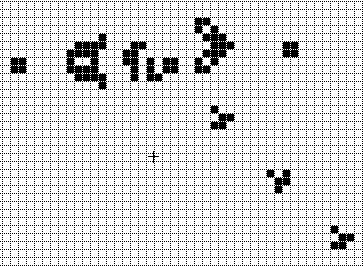
\includegraphics[scale=0.6]{conways.png}
    \end{itemize}
\end{frame}

\begin{frame}{\insertsection}{\insertsubsection}
    \begin{itemize}
        \item weiß bedeutet tot, schwarz bedeutet lebendig
        \item Jede lebende Zelle mit weniger als zwei lebenden Nachbarn stirbt
        \item Jede lebende Zelle mit zwei oder drei lebenden Nachbarn überlebt
        \item Jede lebende Zelle mit mehr als drei lebenden Nachbarn stirbt
        \item Jede tote Zelle mit genau drei Nachbarn wird lebendig
        \item \textbf{Video: Conway's Game of Life}
    \end{itemize}
\end{frame}

\subsection{Grundlagen}
\begin{frame}{\insertsection}{\insertsubsection}
	\begin{itemize}
		\item Self-organized criticality (SOC) ist ein Phänomen bei kontinuierlichen dynamischen
            Systemen
        \pause
        \item Mit der Zeit nähern sich die Parameter des dynamischen Systems einem
            \textbf{kritischen Punkt} an
        \pause
        \item An bestimmten \textbf{kritischen Punkten} findet ein \textbf{Phasenübergang} statt
        \pause
        \item Bei einem \textbf{Phasenübergang} reicht eine geringfügige quantitative Änderung des Systems
            aus, um eine qualitative Änderung des Systems herbeizuführen
        \pause
        \item Der \textbf{kritische Punkt} ist ein Attraktor
        \item Ein \textbf{Attraktor} beschreibt eine Menge von Variablen, die sich mit der Zeit
            einem bestimmten Wert annähern
	\end{itemize}
\end{frame}

\subsection{Phänomenologie}
\begin{frame}{\insertsection}{\insertsubsection}
	\begin{itemize}
		\item Komplexe Strukturen entstehen durch einfache lokale Wechselwirkungen
        \pause
		\item Es ist momentan unmöglich vorherzusagen, ob ein Algorithmus oder System
            SOC-artiges Verhalten aufweist (Simulation erforderlich)
        \pause
        \item Die meisten SOC-Systeme sind zu keinem Zeitpunkt stabil
        \pause
        \item Innerhalb des Einzugsbereichs eines Attraktors führen alle Startparameter zum gleichen
            Ergebnis (\textbf{selbst}organisiert)
        \item Anfangsparameter können in der Regel stark variiert werden, ohne dass sich Endzustand stark ändert
	\end{itemize}
\end{frame}

\section{Sandpile Model}
\subsection{Allgemein}
\begin{frame}{\insertsection}{\insertsubsection}
	\begin{itemize}
        \item Bak-Tang-Wiesenfeld-Modell für Lawinen
        \item Zellulärer Automat auf einem beschränkten Raster
        \pause
        \item Abstrakte Funktionweise:
            \pause
            \begin{itemize}
                \item Zufällige oder zentrale Platzierung von Chips auf dem Raster
                \pause
                \item Anzahl der Chips pro Zelle geben die Höhe an
                \pause
                \item Übersteigt die Zahl der Chips eine Schwelle, teilt die Zelle ihre Chips auf
                    ihre Nachbarn auf
            \end{itemize}
        \item \textbf{Video: Simulation}
        \item \textbf{Video: Experiment}
	\end{itemize}
\end{frame}

\subsection{Algorithmische Funktionsweise}
\begin{frame}[fragile]{\insertsection}{\insertsubsection}
    \footnotesize
    \begin{lstlisting}[language=Python,numbers=left]
iterations = 1000
size = 100
sandpile = [[0 for i in range(size)] for i in range(size)]

while iterations > 0:
    sandpile[size/2-1][size/2-1] += 1
    for x in size:
        for y in size:
            if sandpile[x][y] >= 4:
                sandpile[x][y] -= 4
                sandpile[x-1][y] += 1
                sandpile[x+1][y] += 1
                sandpile[x][y-1] += 1
                sandpile[x][y+1] += 1
    iterations -= 1
    \end{lstlisting}
\end{frame}

\begin{frame}{\insertsection}{\insertsubsection}
    \begin{figure}[p]
        \centering
        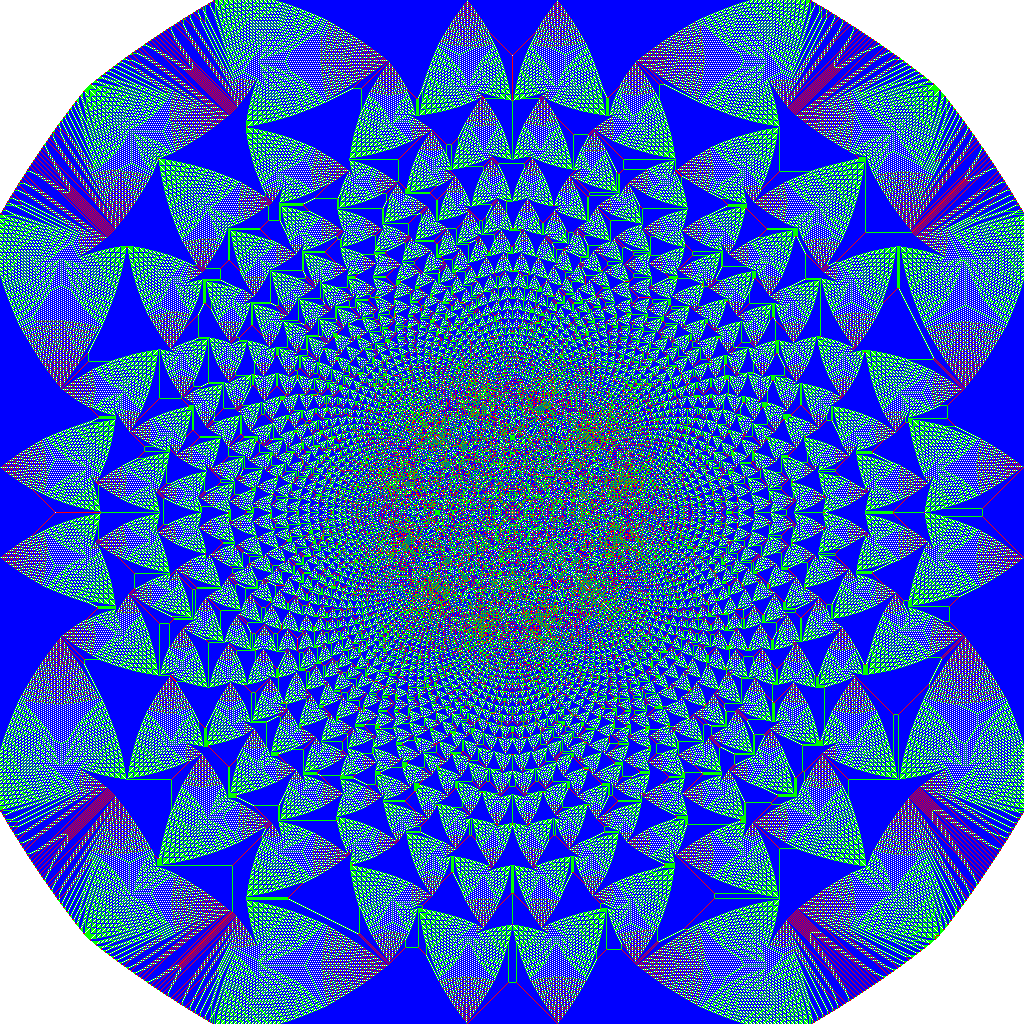
\includegraphics[scale=0.16]{Backtang2.png}
        \caption{Simulation von 28M Sandkörnern}
    \end{figure}
\end{frame}

\subsection{Eindimensionale Sandpile}
\begin{frame}[fragile]{\insertsection}{\insertsubsection}
    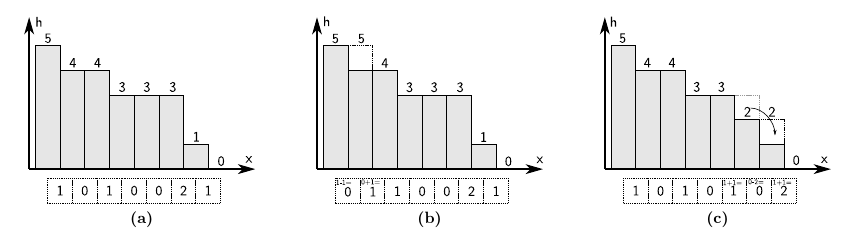
\includegraphics[scale=0.5]{oned.png}
    \begin{itemize}
        \item Zeigt nur kritisches Verhalten ab zwei Dimensionen
        \item Sand wandert nach rechts aus dem System
        \item Eindimensional ist das System ``minimal kritisch''
    \end{itemize}
\end{frame}

\subsection{weitere Eigenschaften}
\begin{frame}[fragile]{\insertsection}{\insertsubsection}
    \begin{itemize}
        \item Wenn ein Sandkorn hinzugefügt wird, kann es sein, dass gar nichts geschieht
        \item Es kann auch sein, dass sich jede Zelle ändert in einer Kettenreaktion
        \item Wie bei SOC typisch, ist der Startzustand ist nicht wichtig
        \item Es ist egal, wo Sandkörner hinzugefügt werden
        \item Etwaige zusätzliche Systemparameter sind auch egal (z.B. Beschaffenheit des Sandes)
    \end{itemize}
\end{frame}

\section{Andere Beispiele}
\subsection{Anwendungen}
\begin{frame}{\insertsection}{\insertsubsection}
	\begin{itemize}
        \item Drossel-Schwabl Modell für Waldbrände
        \pause
        \item Olami–Feder–Christensen Modell für Erdbeben
        \item Bak-Sneppen Modell für Evolution
        \item Landformationen
        \item Boersendynamik
        \item Gehirnsignale
        \item Neutronensternbeben
        \item Solarflares
	\end{itemize}
\end{frame}

\subsection{Drossel-Schwabl Modell für Waldbrände}
\begin{frame}{\insertsection}{\insertsubsection}
	\begin{itemize}
        \item Zellulärer Automat zur Modellierung und Simulation von Waldbränden
        \item Regeln:
        \begin{enumerate}
            \item Eine brennende Zelle wird zu einer leeren Zelle
            \item Ein Baum fängt Feuer, wenn mindestens ein Nachbar brennt
            \item Ein Baum fängt Feuer mit Wahrscheinlichkeit f auch wenn kein Nachbar brennt
            \item In einer leeren Zelle wächst ein Baum mit Wahrscheinlichkeit p
        \end{enumerate}
        \item Modell funktioniert nicht auf großen Maßstäben
        \item \textbf{Video: Experiment}
	\end{itemize}
\end{frame}

\section{Quellen}
\subsection{}
\begin{frame}{\insertsection}{\insertsubsection}
	\begin{itemize}
        \tiny
        \item \url{Bak, P., Tang, C. and Wiesenfeld, K. (1987). "Self-organized criticality: an
            explanation of 1/f noise". Physical Review Letters 59 (4): 381–384.}
        \item \url{https://www.youtube.com/watch?v=-d7\_OGn22d4}
        \item \url{https://www.youtube.com/watch?v=LfJCngN44ug}
        \item \url{https://www.youtube.com/watch?v=OEbCsKJKXaE}
        \item \url{https://www.youtube.com/watch?v=bUd4d8BDIzI}
        \item \url{http://www.douban.com/note/94846105/}
        \item \url{http://mathworld.wolfram.com/ElementaryCellularAutomaton.html}
        \item \url{http://commons.wikimedia.org/wiki/File:Backtang2.png}
	\end{itemize}
\end{frame}


\end{document}
